% THIS IS SIGPROC-SP.TEX - VERSION 3.1
% WORKS WITH V3.2SP OF ACM_PROC_ARTICLE-SP.CLS
% APRIL 2009
%
% It is an example file showing how to use the 'acm_proc_article-sp.cls' V3.2SP
% LaTeX2e document class file for Conference Proceedings submissions.
% ----------------------------------------------------------------------------------------------------------------
% This .tex file (and associated .cls V3.2SP) *DOES NOT* produce:
%       1) The Permission Statement
%       2) The Conference (location) Info information
%       3) The Copyright Line with ACM data
%       4) Page numbering
% ---------------------------------------------------------------------------------------------------------------
% It is an example which *does* use the .bib file (from which the .bbl file
% is produced).
% REMEMBER HOWEVER: After having produced the .bbl file,
% and prior to final submission,
% you need to 'insert'  your .bbl file into your source .tex file so as to provide
% ONE 'self-contained' source file.
%
% Questions regarding SIGS should be sent to
% Adrienne Griscti ---> griscti@acm.org
%
% Questions/suggestions regarding the guidelines, .tex and .cls files, etc. to
% Gerald Murray ---> murray@hq.acm.org
%
% For tracking purposes - this is V3.1SP - APRIL 2009

\documentclass{acm_proc_article-sp}

\usepackage[utf8]{inputenc}
\usepackage[brazilian]{babel}
\usepackage{color}
\usepackage{listings}
\usepackage{textcomp}

%\usepackage{url}
\usepackage[colorlinks]{hyperref}
\definecolor{darkblue}{rgb}{0,0,0.5}
\hypersetup{ colorlinks=true, urlcolor=darkblue, linkcolor=darkblue, citecolor=darkblue }

%\usepackage{algorithm2e}
\hyphenation{BigBlueButton}
\newcommand{\todo}[1]{\textcolor[rgb]{1.00,0.00,0.00}{\bf \uppercase{#1}}}

\begin{document}

\title{Mconf-Mobile: videoconferência \\BigBlueButton no Android}
%
% You need the command \numberofauthors to handle the 'placement
% and alignment' of the authors beneath the title.
%
% For aesthetic reasons, we recommend 'three authors at a time'
% i.e. three 'name/affiliation blocks' be placed beneath the title.
%
% NOTE: You are NOT restricted in how many 'rows' of
% "name/affiliations" may appear. We just ask that you restrict
% the number of 'columns' to three.
%
% Because of the available 'opening page real-estate'
% we ask you to refrain from putting more than six authors
% (two rows with three columns) beneath the article title.
% More than six makes the first-page appear very cluttered indeed.
%
% Use the \alignauthor commands to handle the names
% and affiliations for an 'aesthetic maximum' of six authors.
% Add names, affiliations, addresses for
% the seventh etc. author(s) as the argument for the
% \additionalauthors command.
% These 'additional authors' will be output/set for you
% without further effort on your part as the last section in
% the body of your article BEFORE References or any Appendices.

\numberofauthors{1} %  in this sample file, there are a *total*
% of EIGHT authors. SIX appear on the 'first-page' (for formatting
% reasons) and the remaining two appear in the \additionalauthors section.
%
\author{
% You can go ahead and credit any number of authors here,
% e.g. one 'row of three' or two rows (consisting of one row of three
% and a second row of one, two or three).
%
% The command \alignauthor (no curly braces needed) should
% precede each author name, affiliation/snail-mail address and
% e-mail address. Additionally, tag each line of
% affiliation/address with \affaddr, and tag the
% e-mail address with \email.
%
% 1st. author
%\alignauthor
Felipe Cecagno,
Valter Roesler\\
       \affaddr{Instituto de Informática}\\
       \affaddr{Universidade Federal do Rio Grande do Sul}\\
       \affaddr{Porto Alegre, Rio Grande do Sul, Brasil}\\
       \email{\{fcecagno, roesler\}@inf.ufrgs.br}
}
\date{24 de julho de 2011}

\maketitle
\begin{resumo}
  Este artigo apresenta um dos resultados desenvolvidos no projeto Mconf. O Mconf-Mobile é um aplicativo de código aberto para dispositivos móveis com sistema operacional Android. Ele permite interação entre usuários de smartphones e tablets com usuários de computadores de mesa através do sistema de webconferência BigBlueButton. Serão apresentados alguns objetivos do projeto, a arquitetura da solução e suas principais funcionalidades.
\end{resumo}

\begin{abstract}
  This article presents a result of the Mconf project. The Mconf-Mobile is an application for mobile devices with Android operational system. It makes possible to interact with other users in a BigBlueButton videoconference. We present some goals of the project, the solution's architecture and its main functionalities.
\end{abstract}

% http://www.acm.org/about/class/ccs98-html
% A category with the (minimum) three required fields
%\category{}{Peer-to-peer multimedia systems and streaming}{}
%\category{}{Software development using multimedia techniques}{}
%\category{H.4}{Information Systems Applications}{Miscellaneous}


\category{C.3}{Special-purpose and application-based systems: }{Real-time and embedded systems}
%\category{J.7}{Computers in other systems}{Real time}
%\category{I.6}{Simulation and modeling}{Applications}
\category{H.4}{Information systems applications}{Communications Applications: }{Computer conferencing, teleconferencing, and videoconferencing}

%\terms{Design, Experimentation}

\keywords{Videoconferência, Android, BigBlueButton, Código aberto, Mconf}

\section{Introdução}

Dispositivos móveis inteligentes vêm ganhando a cada dia mais espaço e popularidade. A troca de telefones celulares ``burros'' por smartphones acontece por diversos motivos, e um deles é a grande variedade de aplicativos disponíveis. Dentre eles, os mais populares são os aplicativos de entretenimento~\cite{android-stats}, categoria que inclui os jogos, que aproveitam a capacidade de processamento dos dispositivos e oferecem distração aos usuários.

Além dos jogos, aplicações de vídeo em tempo real vêm crescendo no mercado de aplicativos. Clientes VoIP\footnote{\emph{Voice over IP}, ou Voz sobre IP} como o Sipdroid e aplicativos populares por sua versão para desktop como o Skype já incluem a funcionalidade de videochamada nos seus aplicativos para dispositivos móveis. Além destes, o Fring permite chamada em grupos de até quatro pessoas.

Entretanto, tanto o Skype quanto o Fring permitem chamadas apenas para clientes de mesmo tipo, ou seja, Skype se comunica com Skype e Fring se comunica com Fring, mas não existe interação entre eles. Os clientes VoIP são mais genéricos, mas ao mesmo tempo mais limitados quanto a funcionalidades.

O principal objetivo do projeto Mconf é proporcionar uma solução de código aberto para webconferência com foco na facilidade de uso e integração com dispositivos móveis e redes sociais\footnote{\url{http://inf.ufrgs.br/prav/gtmconf}}. A solução integra o sistema de webconferência BigBlueButton~\cite{bigbluebutton} com o portal web em forma de rede social Global Plaza, e prevê interação com dispositivos móveis através do Mconf-Mobile.

O projeto Mconf é desenvolvido pelo Laboratório de Projetos em Áudio e Vídeo da Universidade Federal do Rio Grande do Sul, teve início em novembro de 2010 e é financiado pela Rede Nacional de Ensino e Pesquisa no âmbito do programa de Grupos de Trabalho da RNP.

O código-fonte do Mconf-Mobile está disponível em um repositório público\footnote{\url{https://github.com/mconf/mconf-mobile}} e é licenciado sob a \emph{GNU General Public License}. O aplicativo está disponível para \emph{download} no Google Code do projeto\footnote{\url{http://code.google.com/p/mconf/}} e futuras versões serão disponibilizadas gratuitamente na loja oficial do Android.

%O objetivo do subprojeto Mconf-Mobile é desenvolver um aplicativo para videoconferência integrado ao ambiente BigBlueButton. Com isso visa-se a interação plena entre dispositivos móveis e clientes desktop conectados ao sistema através da web.

\section{Arquitetura}\label{sec:arquitetura}

Conforme descrito anteriormente, o Mconf integra dois sistemas existentes de código aberto voltados para videoconferência: o BigBlueButton e o Global Plaza. Entretanto, o aplicativo Android se comunica diretamente com o BigBlueButton e não realiza qualquer interação com o Global Plaza. Isso se deve a uma decisão estratégica de projetar o Mconf-Mobile como o cliente Android oficial do BigBlueButton. Dessa forma, usuários do BigBlueButton podem utilizar o aplicativo independente do portal web do Mconf. Tal decisão fez o projeto ganhar visibilidade e atrair a atenção da comunidade de desenvolvedores do BigBlueButton (que conta com mais de 950 membros\footnote{\url{http://groups.google.com/group/bigbluebutton-dev/about}}).

O BigBlueButton é um sistema de código aberto para webconferência voltado principalmente para ensino à distância. Ele oferece funcionalidades como interação por áudio, vídeo e bate-papo (público e privado), além de compartilhamento da tela do computador e apresentação síncrona de slides e documentos.

O cliente web para desktop é desenvolvido na plataforma Adobe Flash e toda a comunicação com o servidor é feita através do protocolo proprietário RTMP\footnote{\emph{Real-Time Messaging Protocol}}. Já o servidor do BigBlueButton utiliza o Red5\footnote{\url{http://www.red5.org/}}, que é uma implementação livre do Adobe Flash Media Server. Além da comunicação por vídeo, realizada de forma transparente entre o cliente Flash e o servidor Red5, são utilizados \emph{Remote Shared Objects} (RSO) e \emph{Remote Procedure Calls} (RPC) para as demais trocas de mensagens, como bate-papo e gerenciamento de status de participantes.

Para áudio, o sistema utiliza um servidor VoIP, que pode ser tanto o FreeSWITCH quanto o Asterisk. No cliente web é utilizada uma implementação de telefone SIP\footnote{\emph{Session Initiation Protocol}} em Flash.

Apesar do Android oferecer suporte a plataforma Flash a partir da sua versão 2.2, optou-se por desenvolver um aplicativo nativo através da SDK padrão do Android para permitir compatibilidade com as versões anteriores. A arquitetura do aplicativo será detalhada nas subseções seguintes.

\subsection{Flazr}

Toda a comunicação RTMP entre o aplicativo e o servidor Red5 é feita através da biblioteca Flazr, uma implementação livre em Java de protocolos de \emph{streaming} multimídia\footnote{\url{http://flazr.com}}. A biblioteca implementa partes importantes do protocolo RTMP, como por exemplo o \emph{handshake} inicial e multiplexação/demultiplexação de mensagens de controle, áudio e vídeo, comandos de RPC e controle de fluxos de dados.

Entretanto, a biblioteca não oferece suporte a RSO, recurso indispensável para realização plena da comunicação com o servidor. Por exemplo, informações de entrada e saída de participantes, presença de vídeo de um determinado participante ou pedido de atenção através do recurso ``levantar a mão'' são ações informadas através do objeto \textbf{participantsSO}. Outro exemplo é a troca de mensagens públicas de bate-papo, que é realizada através do objeto \textbf{chatSO}. 

Por isso, o suporte a RSO teve de ser adicionado à biblioteca. A implementação de gerência de objetos compartilhados e da multiplexação/demultiplexação de mensagens teve como base o código do Red5 e a especificação do protocolo RTMP~\cite{rtmp}.

\subsection{BBB-Java}

O BBB-Java é a biblioteca responsável pela interação entre um aplicativo genérico em Java e um servidor BigBlueButton. Essa biblioteca foi desenvolvida pelo projeto Mconf para ser utilizada no Mconf-Mobile, mas buscou-se manter um baixo acoplamento entre a biblioteca e o aplicativo Android exatamente para possibilitar e incentivar o desenvolvimento de novos aplicativos não-web integrados ao sistema de webconferência. Além disso, a biblioteca pode ser utilizada na criação de aplicativos robôs que auxiliem a realização de testes de funcionamento e de carga.

Dentre os recursos oferecidos pela biblioteca estão:
\begin{itemize}
 \item Gerenciamento de salas de conferência (pesquisa das salas existentes, criação de novas salas e acesso a uma sala específica);
 \item Atualização do status dos participantes da sessão;
 \item Troca de mensagens de bate-papo (público e privado);
 \item Recepção e envio de dados de vídeo.
\end{itemize}

O gerenciamento de salas de conferência é feito através de chamadas a um aplicativo web JSP (\emph{mobile.jsp}), desenvolvido no projeto Mconf, que utiliza a API do BigBlueButton para executar as funções citadas. Um aplicativo intermediário é necessário, pois a API do BigBlueButton utiliza um \emph{security salt} alfanumérico de 32 caracteres para gerar um \emph{checksum} de cada requisição. Esse \emph{salt} é conhecido apenas no ambiente web, não em aplicações externas como é o caso do BBB-Java, e não é plausível que um aplicativo exija do usuário uma senha de 32 dígitos para acesso a um servidor.

Inicialmente, em caráter experimental, o \emph{mobile.jsp} removia a necessidade do \emph{salt}. Essa brecha de segurança foi solucionada quando um novo \emph{salt} de apenas 5 caracteres foi implantado, tornando factível a entrada desse dado pelo usuário.

Os demais recursos são oferecidos pela biblioteca através de uma comunicação RTMP com o servidor Red5. Para tal utilizou-se a versão modificada da biblioteca Flazr, com suporte a RSO.

\subsection{BBB-Android}\label{subsec:bbb-android}

O BBB-Android é o aplicativo Android que utiliza o BBB-Java para interação com o servidor BigBlueButton. Esse aplicativo foi escrito principalmente em Java, utilizando o \emph{Software Development Kit} (SDK) padrão do Android, e uma pequena parte crítica em desempenho foi desenvolvida em C/C++ com o \emph{Native Development Kit} (NDK).

Considerando que o servidor BigBlueButton utiliza um servidor VoIP para lidar com os fluxos de áudio, para o BBB-Android adotou-se a estratégia de integrar ao aplicativo uma solução existente de VoIP de código aberto. Optou-se pelo aplicativo Sipdroid\footnote{\url{https://market.android.com/details?id=org.sipdroid.sipua}}, um dos telefones SIP mais populares do Android Market, adicionando assim a funcionalidade de interação por áudio. Dentre os codecs suportados pelo Sipdroid está o Speex, codec padrão de áudio do BigBlueButton, implementado na linguagem C e compilado através do NDK.

O codec de vídeo padrão utilizado no BigBlueButton é o H.263, e a estratégia de solução foi a mesma do Sipdroid. Optou-se por utilizar uma compilação otimizada da biblioteca FFmpeg\footnote{\url{http://www.ffmpeg.org/}} para Android, gerada através do NDK, que tivesse apenas esse codec habilitado. O FFmpeg é uma biblioteca escrita na linguagem C que implementa diversos codificadores e decodificadores de áudio e vídeo.

\section{Principais funcionalidades}

A figura~\ref{fig:mconf-mobile} ilustra as principais funcionalidades do aplicativo, que serão descritas nesta seção.

\begin{figure}[htp]
\centering
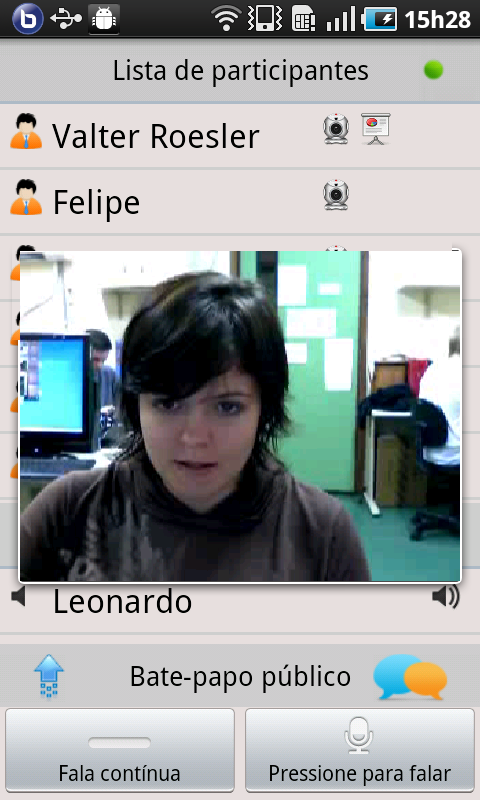
\includegraphics[width=45mm]{app1.png}
\caption{Tela principal do Mconf-Mobile}\label{fig:mconf-mobile}
%\caption{Tela principal do Mconf-Mobile: no centro, o vídeo de um participante sendo exibido; ao fundo, lista dos participantes da sessão e lista dos participantes da conferência de voz; na parte inferior, bate-papo público deslizante e botões de controle de áudio do dispositivo}\label{fig:mconf-mobile}
\end{figure}

\subsection{Bate-papo}

Assim como o cliente web do BigBlueButton, o aplicativo possui a funcionalidade de bate-papo, que pode ser público ou privado. O bate-papo público pode ser observado na figura~\ref{fig:mconf-mobile} como uma barra deslizante, que com um toque do usuário encobre a lista de participantes e deixa visíveis todas as mensagens trocadas (juntamente com o originador da mensagem e horário) e uma caixa de texto para envio de novas mensagens.

Já o bate-papo privado é acessado com um toque do usuário sobre o nome do participante com o qual ele deseja iniciar uma conversa. Uma nova tela é aberta, com as mesmas características do bate-papo público, mas com a particularidade de que somente aquele usuário terá acesso à conversação.

\subsection{Áudio}

O áudio é parte fundamental da interação em um ambiente de videoconferência, logo essa importância é refletida na interface principal do aplicativo. Ao habilitar a conferência de áudio através do botão \textbf{Menu} do aparelho, dois botões aparecem na parte inferior da interface (ver figura~\ref{fig:mconf-mobile}: ``Fala contínua'' e ``Pressione para falar'').

Os botões de controle de áudio são indispensáveis para uma interação de qualidade, pois experimentalmente verificou-se que o microfone de dispositivos móveis é muito sensível a ruído. Além disso, a utilização do botão ``Pressione para falar'' atenua problemas de eco acústico que podem ocorrer se o usuário não utilizar fones de ouvido.

Através do menu também é possível habilitar o alto-falante do dispositivo, ajustar controle de volume e ganho do microfone, e também encerrar a conferência de áudio.

\subsection{Vídeo}

%O recurso de vídeo, presente no cliente web do BigBlueButton, também é explorado no aplicativo Android. Como pode ser visto na figura~\ref{fig:mconf-mobile}, um ícone em forma de webcam informa se o usuário possui ou não sua câmera habilitada. Através de um toque longo sobre o nome do participante com vídeo habilitado, o usuário pode escolher a opção de exibição do vídeo. Ao fazê-lo, uma tela sobreposta com o vídeo do participante é exibida.

O recurso de vídeo, presente no cliente web do BigBlueButton, também é explorado no aplicativo Android. Como pode ser visto na figura~\ref{fig:mconf-mobile}, um ícone em forma de webcam informa se o participante possui sua câmera habilitada. Um toque longo sobre o nome deste participante faz aparecer um menu com a opção ``Exibir vídeo''. Ao selecioná-la, o vídeo do participante é exibido em uma tela sobreposta.

\subsection{Gerência de conferência}

Caso o usuário entre na sessão como \textbf{Moderador}, é possível realizar uma série de operações administrativas, como promover um participante a Apresentador, colocar em mudo um participante que esteja emitindo ruído, abaixar a mão de um participante que pediu atenção e até expulsar um participante da sessão. 

Esses recursos sugerem um novo caso de uso para o aplicativo: um professor utiliza o quadro negro para uma exposição aos seus alunos que estão remotamente conectados; ele não permanece em frente ao seu computador durante a exposição, mas pode utilizar um dispositivo móvel como controle remoto para gerenciar a videoconferência (checar mensagens de bate-papo, atender a um pedido de atenção, etc.).

%Esses recursos sugerem um novo caso de uso para o aplicativo, em que o moderador da sessão (por exemplo, um professor em uma videoaula) não permanece em frente ao computador e utiliza um dispositivo móvel como controle remoto para gerenciar a videoconferência.

\section{Conclusão}

Este artigo apresentou o Mconf-Mobile, um aplicativo para videoconferência em dispositivos móveis com sistema operacional Android. A principal contribuição do projeto Mconf é o desenvolvimento em código aberto de uma solução completa de videoconferência que integra dispositivos móveis e redes sociais. O desenvolvimento modular, conforme apresentado na seção~\ref{sec:arquitetura}, permite que as partes de software produzidas sejam utilizadas em outros projetos de forma independente.

Novas funcionalidades estão previstas para o futuro, como captura de vídeo a partir de um dispositivo móvel, possibilidade de visualização de vários vídeos ao mesmo tempo, integração do módulo de apresentação do BigBlueButton ao aplicativo e desenvolvimento de um novo módulo que permita edição cooperativa de texto através de um bloco de notas. 

%
% The following two commands are all you need in the
% initial runs of your .tex file to
% produce the bibliography for the citations in your paper.
\bibliographystyle{abbrv}
\bibliography{paper}  % sigproc.bib is the name of the Bibliography in this case
% You must have a proper ".bib" file
%  and remember to run:
% latex bibtex latex latex
% to resolve all references
%
% ACM needs 'a single self-contained file'!
%
\balancecolumns
% That's all folks!
\end{document}
